% Copyright (C) 2010,2011,2012 The ESPResSo project
% Copyright (C) 2002,2003,2004,2005,2006,2007,2008,2009,2010 
%   Max-Planck-Institute for Polymer Research, Theory Group
%  
% This file is part of ESPResSo.
%   
% ESPResSo is free software: you can redistribute it and/or modify it
% under the terms of the GNU General Public License as published by the
% Free Software Foundation, either version 3 of the License, or (at your
% option) any later version.
%  
% ESPResSo is distributed in the hope that it will be useful, but
% WITHOUT ANY WARRANTY; without even the implied warranty of
% MERCHANTABILITY or FITNESS FOR A PARTICULAR PURPOSE.  See the GNU
% General Public License for more details.
%  
% You should have received a copy of the GNU General Public License
% along with this program.  If not, see <http://www.gnu.org/licenses/>.
%
\documentclass[
a4paper,                        % paper size
11pt,                           % font size
twoside,                        % two sided
footsepline,                    % add a line to separate the footer
headsepline,                    % add a line to separate the header
headexclude,                    % header does not belong to the text
footexclude,                    % footer does not belong to the text
pagesize,                       % set the pagesize in a DVI document
]{scrartcl}

% Copyright (C) 2010,2011,2012,2013,2014,2015,2016 The ESPResSo project
% Copyright (C) 2002,2003,2004,2005,2006,2007,2008,2009,2010
%  Max-Planck-Institute for Polymer Research, Theory Group
%  
% This file is part of ESPResSo.
%   
% ESPResSo is free software: you can redistribute it and/or modify it
% under the terms of the GNU General Public License as published by the
% Free Software Foundation, either version 3 of the License, or (at your
% option) any later version.
%  
% ESPResSo is distributed in the hope that it will be useful, but
% WITHOUT ANY WARRANTY; without even the implied warranty of
% MERCHANTABILITY or FITNESS FOR A PARTICULAR PURPOSE.  See the GNU
% General Public License for more details.
%  
% You should have received a copy of the GNU General Public License
% along with this program.  If not, see <http://www.gnu.org/licenses/>.
%
\usepackage[draft]{varioref}    % defines \vref
\usepackage{hyperref}           % automatically creates links when
                                % using pdflatex, defines \url
\usepackage{ifpdf}              % defines \ifpdf
\usepackage{graphicx}           % handles graphics
\usepackage{color}              % use colors

\usepackage{amsmath}

\usepackage{verbatim}           % required for \verbatim and \endverbatim
\usepackage{fancyvrb}
\usepackage{calc}               % compute length
\usepackage{ifthen}             % provide ifthen
\usepackage{xspace}
\usepackage{units}
\usepackage[numbers]{natbib}

\usepackage{listings}

% For building the distribution docs, disable todo boxes.
%\usepackage[disable]{todonotes}
\usepackage{todonotes}

\newcommand{\es}{\mbox{\textsf{ESPResSo}}\xspace}
\newcommand{\ie}{\textit{i.e.}\xspace}
\newcommand{\eg}{\textit{e.g.}\xspace}
\newcommand{\etal}{\textit{et al.}\xspace}

\newcommand{\codebox}[1]%
{\texttt{#1}}

\DefineVerbatimEnvironment{code}{Verbatim}%
{commandchars=\\\{\}}
\makeatletter
\newenvironment{tclcode}
{%
  \addtolength{\linewidth}{-2em}% set the line length
  \@minipagetrue%%%DPC%%%
  \@tempswatrue%%%DPC%%%
  \hsize=\linewidth%
  \setbox0=\vbox\bgroup\verbatim
}{\endverbatim
  \unskip\setbox0=\lastbox%%%DPC%%%
  \egroup
  \par%
  \noindent\hspace{1em}%
  \codebox{\box0}%
  \par\noindent%
}
\makeatother

% \newcommand{\todo}[1]{
%   \marginpar{%
%     \setlength{\fboxrule}{1pt}
%     \fcolorbox{red}{yellow}{%
%       \parbox{\marginparwidth-2\fboxrule-2\fboxsep}{%
%         \bf\raggedright\scriptsize #1%
%       }%
%     }%
%   }%
% }

\makeatletter
\renewcommand{\minisec}[1]{\@afterindentfalse \vskip 1.5ex
  {\parindent \z@
    \raggedsection\normalfont\sffamily\itshape\nobreak#1\par\nobreak}%
  \@afterheading}
\makeatother

\newcommand{\esptitlehead}{
  \titlehead{
    \begin{center}
      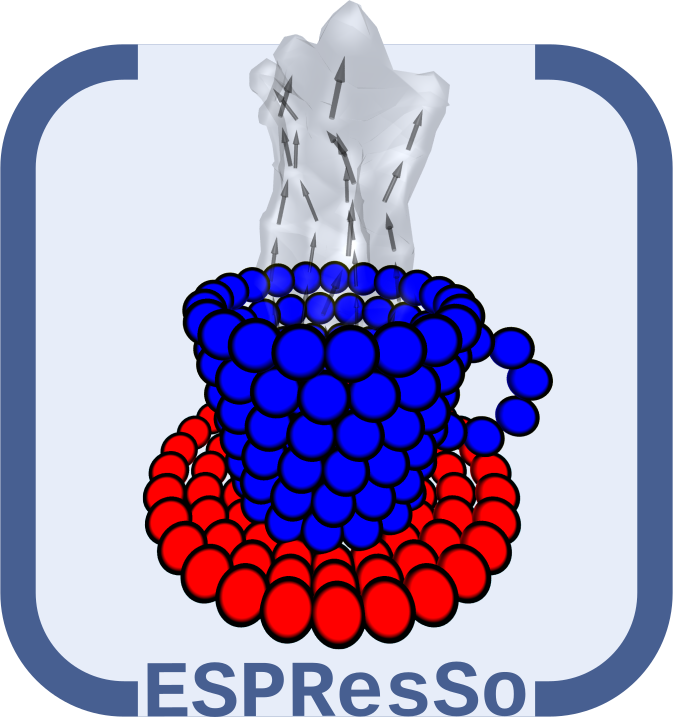
\includegraphics[width=5cm]{logo/logo.pdf}
    \end{center}
  }
}

% Do magic that \bfseries for keywords actually works
\DeclareFontShape{OT1}{cmtt}{bx}{n}{<5><6><7><8><9><10><10.95><12><14.4><17.28><20.74><24.88>cmttb10}{}

% Custom colors
\definecolor{stringblue}{rgb}{0.09,0.211,0.57}
\definecolor{codered}{rgb}{0.655,0.1137,0.3747}
\definecolor{deepgreen}{rgb}{0,0.5,0}
\definecolor{commentgray}{rgb}{0.4,0.4,0.4}
\definecolor{framegray}{rgb}{0.8,0.8,0.8}

% Python style for highlighting
\newcommand\pythonstyle{\lstset{
    language=Python,
    belowskip=\bigskipamount,
    aboveskip=\bigskipamount,
    basicstyle=\ttfamily\small,
    otherkeywords={self},             % Add keywords here
    keywordstyle=\bfseries\color{codered},
    emph={MyClass,__init__},          % Custom highlighting
    emphstyle=\bfseries\color{deepgreen},    % Custom highlighting style
    commentstyle=\color{commentgray}\ttfamily,
    stringstyle=\color{stringblue},
    frame=tb,                         % Any extra options here
    rulecolor=\color{framegray},
    showstringspaces=false            % 
    }
}


% Python environment
\lstnewenvironment{python}[1][]{\pythonstyle \lstset{#1}}{}

% Python for external files
\newcommand\pythonexternal[2][]{{\pythonstyle \lstinputlisting[#1]{#2}}}

% Python for inline
\newcommand\pythoninline[1]{{\pythonstyle\lstinline!#1!}}




%% Grafikpakete
\usepackage{graphicx}%
\usepackage{verbatim}

% How to diplay ESPResSo commands in flowing text. Larger code segments
% should be put inside boxes.
\newcommand{\EScmd}[1]{\texttt{\textbf{#1}}}

% The code block
%\newcommand{\EScode}[1]{ \parbox{0.95\textwidth}{\texttt{#1}}}
\usepackage{listings} 
\lstset{numbers=left, numberstyle=\tiny, numbersep=5pt, showspaces=false, showstringspaces=false,postbreak=\space, breakindent=5pt, breaklines}
\lstset{language=tcl, keywordstyle=\color{blue}\bfseries ,emphstyle=\color{green}, commentstyle=\color{red}\itshape }
\lstset{keywordsprefix=setmd}
\lstset{keywords=[6]{thermostat,part,inter,integrate,rescale_velocities,code_info,save_sim,writepdb,analyze,uwerr}}

\newtheorem{task}{Task}

\begin{document}

\esptitlehead

\title{Tutorial 2: Simple Charged Systems%
\ifdefined\esversion%
\thanks{For \es \esversion}%
\fi%
}
\subtitle{Beyond the \es{} Basics}
\author{? ? \and ? ? \and ? ? \and J. de Graaf}

\maketitle
\tableofcontents

\section{Introduction}

This tutorial expands upon the \es{} features demonstrated in the Lennard-Jones tutorial, by constructing a simulation script that is used for studying a simple 1:1 electrolyte, i.e., a suspension of monovalent ions. For information on the Tcl commands, we refer to the L-J tutorial; however, most of the constructs should be self-explanatory. We assume that the reader is familiar with the basic concepts of a MD simulation here. The code pieces in the tutorial can be directly copied into a script file, which then can be run using the command \verb|Espresso <script>| invoked from the \es{} source directory.

\textbf{N.B. The script can be placed in the \es{} main directory or any of the subdirectories to allow evaluation, i.e., \texttt{Espresso <dir/subdir/script>}. However, it is currently set up such that the output is directed to a \texttt{data} folder in your \es{} main directory. If this folder is not present yet, you can create it, or change the script(s) to output the data elsewhere.}

\section{The Basic Set Up}

As in the L-J tutorial, our script starts by setting up the initial configuration. It is convenient to specify the density and the number of particles\footnote{The number of particles is assumed to be even in this tutorial, because of the way we set up the charges in the box. Remember, the system must be charge neutral.} of the system as parameters:

{\small\vspace{0,2cm}
\begin{lstlisting}{bsp_code}
set n_part 200
set density 0.7
set box_l [expr pow($n_part/$density,1./3.)]
\end{lstlisting}\vspace{0,2cm}
}

\noindent These variables do not change anything in the simulation engine, since we did not invoke the \verb|setmd| command; they are just standard Tcl variables. This way of writing the script increases the readability and flexibility of the script. The box length is not an explicitly parameter of this simulation, it is calculated from the number of particles and the system density. This allows one to change the parameters more easily later, e.g., to simulate a bigger system.
 
As mentioned, the parameters of the simulation engine are modified by the \verb|setmd| command. We now use this command to set a cubic box for the simulation with size \verb|box_l| and we fill it with particles

{\small\vspace{0,2cm}
\begin{lstlisting}[firstnumber= auto]{bsp_code}
setmd box_l $box_l $box_l $box_l

t_random seed 12345
set q 1
set type 0
for {set i 0} { $i < $n_part } {incr i} {
  set posx [expr $box_l*[t_random]]
  set posy [expr $box_l*[t_random]]
  set posz [expr $box_l*[t_random]]
  set q [expr -$q]
  set type [expr 1-$type]
  part $i pos $posx $posy $posz q $q type $type
}
\end{lstlisting}\vspace{0,2cm}
}

\noindent This loop adds \verb|n_part| particles at random positions (using the \es{} internal random number generator), one by one. In this construct, only two commands are not standard Tcl commands: the random number generator \verb|t_random| and the \verb|part| command. The latter is used to specify particle properties: the number, the position, the charge \verb|q|, and the \verb|type|. In \es{} the particle type is just an integer number, which allows for grouping of the particles, it does not imply any physical parameters. This grouping enables the user to define different interactions between the various particles. Here positive charges have type 0, negative charges have type 1. Note that we interchange the type and charge for each particle we add to the box\footnote{We have set up a charge neutral box with oppositely charged particles, i.e., we simulate a restricted primitive-model electrolyte.}. 

Now that the particles are set, we define the ensemble in which we will be simulating. This is done using the \verb|thermostat| command. The system is simulated in the $NVT$ (isothermal-isochoric) ensemble. We also set some integration scheme parameters:

{\small\vspace{0,2cm}
\begin{lstlisting}[firstnumber= auto]{bsp_code}
setmd time_step 0.01
setmd skin 0.3
set temp 1.0
set gamma 1.0
thermostat langevin $temp $gamma
\end{lstlisting}\vspace{0,2cm}
}

\noindent The above command switches on the Langevin thermostat for the $NVT$ ensemble, with temperature \verb|temp| and friction coefficient \verb|gamma|. The skin depth \verb|skin| is a parameter for the link-cell system, as mentioned in the L-J tutorial. Note that we did not set up the \verb|cellsystem| in this script; the \texttt{cellsystem domain\_decomposition} option is default in \es{}.

\vspace{1cm}
\framebox{
\begin{minipage}{0.95\textwidth} 
\begin{task}
Look up what the friction coefficient $\gamma$ does for the Langevin thermostat and experiment with different values, to see what the effects on your simulation results are. Also examine the effects of the skin size on your simulation's performance.\newline

Hint: examine the relevant passages in the book by Frenkel and Smit~\cite{frenkel02b}, as well as the User Guide.
\end{task}
\end{minipage}}
\vspace{1cm}

Before we can start the simulation, we have to specify the interactions between our particles. We use a simple, purely repulsive Lennard-Jones interaction to model the hard-core repulsion, i.e., the Weeks-Chandler-Andersen (WCA) potential. This hard-core is required to prevent opposite charges from forming charge neutral pairs with zero inter-particle distance. The charges interact via the Coulomb potential:

{\small\vspace{0,2cm}
\begin{lstlisting}[firstnumber= auto]{bsp_code}
set sig 1.0
set cut [expr 1.12246*$sig]
set eps 1.0
set shift [expr 0.25*$eps]

inter 0 0 lennard-jones $eps $sig $cut $shift 0.0
inter 1 0 lennard-jones $eps $sig $cut $shift 0.0
inter 1 1 lennard-jones $eps $sig $cut $shift 0.0

puts [inter coulomb 10.0 p3m tunev2 accuracy 1.0e-3 mesh 32]
\end{lstlisting}\vspace{0,2cm}
}

\noindent The first three \verb|inter| commands instruct \es\ to use the same WCA potential for the interaction between all combinations of the two particle types 0 and 1. By setting different parameters for different combinations, one could simulate a system with a size asymmetry. The last line sets the Bjerrum length ($\lambda_{B}$) to the value $(\lambda_{B} = 10)$\footnote{A value of $\lambda_{B} = 10$ is fairly high. In our primitive model system, this will lead to the particles interacting strongly with each other. However, for these densities we are still in the liquid phase~\cite{smit}.}, and then instructs \es{} to use the P$^3$M algorithm, by which the Coulomb interactions between particles can be efficiently determined. This algorithm is set to try to find suitable parameters for a root-mean-square force error lower than $10^{-3}$, with a fixed mesh size of 32. The mesh is fixed here to speed up the tuning; for a `real' simulation, one would also tune this parameter. The \verb|puts| statement ensures that parameters that the tuning found are returned. 

The tuning takes some time. If you run many simulations with the same parameters, it is useful to calculate the P$^3$M parameters once, save them, and load them before running subsequent simulations. You can obtain the P$^3$M parameters by \verb|inter coulomb|:

{\vspace{0,2cm}\small
\begin{lstlisting}[numbers=none]
set p3m_params [inter coulomb]
foreach f $p3m_params { eval inter $f }
\end{lstlisting}\vspace{0,2cm}
}

\noindent They are printed in a format suitable to feed them back to the \verb|inter| command. This is accomplished in the second line. Note that when you print \verb|p3m_params| to the screen, you will find that it consists of two lists. The first list sets the `internal' parameters, the second list sets the boundary conditions. To ensure that both parameter sets are properly passed back to the \verb|inter| environment, the list are individually past using the \verb|foreach| command.

\vspace{1cm}
\framebox{
\begin{minipage}{0.95\textwidth} 
\begin{task}
Examine the output of the \texttt{inter coulomb} command and figure out what every element of the P$^{3}$M parameter set does.\newline

Hint: Examine the User Guide and the relevant papers, Refs.~\cite{Hockney,deserno1,deserno2,ballenegger}.
\end{task}
\end{minipage}}
\vspace{1cm}

Finally, we determine the degrees of freedom that are available to the particles. This number is dependent on the in-compiled features of \es{} and can be determined in the following way\footnote{There also exists a predefined tcl function \texttt{degrees\_of\_freedom} which does the same.}: 

{\small\vspace{0,2cm}
\begin{lstlisting}[firstnumber= auto]{bsp_code}
if { [regexp "ROTATION" [code_info]] } {
  set deg_free 6
} else {
  set deg_free 3
}
\end{lstlisting}\vspace{0,2cm}
}

\noindent In \es{} there are usually 3 translational degrees of freedom per particle. However, if the \verb|ROTATION| option is compiled in, there are 3 additional degrees of freedom, associated with the the rotations of the particle. These also contribute to the kinetic energy. This is important if we want to calculate the `kinetic temperature', i.e., the temperature equivalent of the kinetic energy, via the equipartition theorem.

\section{Running the Simulation}

Now that we have set up the system, we can warm it to prevent the initial energies from becoming too high using the \verb|forcecap| command. \textbf{N.B. The command in versions of \es{} predating the 3.1.1 release is \lstinline|inter ljforcecap| Please adjust your script according to the version you are using.} This warming is necessary since we placed the particles at random positions in the box, therefore same-sign charges may be very close together, leading to extremely high forces.

{\small\vspace{0,2cm}
\begin{lstlisting}[firstnumber= auto]{bsp_code}
set tcl_precision 8
set integ_steps 200
puts "Warming loop"

for {set cap 20} {$cap < 200} {incr cap 20} {
  inter forcecap $cap
  integrate $integ_steps
  puts -nonewline "t = [setmd time], E = [analyze energy total] \r"
  flush stdout
}

puts "\n"
inter forcecap 0
\end{lstlisting}\vspace{0,2cm}
}

\noindent Note that we set the initial force capping to 20 and increase this every 200 integration steps by 20, until the capping value has reached 200. We output the time and energy for each of these cycles, to monitor the process. If the system was insufficiently (or not at all) warmed \es{} will likely give the error message: \texttt{particle coordinate out of range}. The final command switches the force capping off.

Next it is necessary to equilibrate the system, before we can begin any production run. Remember, the system has only just reached the non-force-capped state, and needs to relax before we can sample. 

\vspace{1cm}
\framebox{
\begin{minipage}{0.95\textwidth} 
\begin{task}
Determine the correct number of equilibration integration steps by examining the physical quantities that are relevant to our system.\newline

Hint: consider the kinetic temperature, as discussed above, or the total energy.
\end{task}
\end{minipage}}
\vspace{1cm}

\noindent A possible way of determining the length of the equilibration is using this code block.

{\small\vspace{0,2cm}
\begin{lstlisting}[firstnumber= auto]{bsp_code}
set en [open "data/equilibration.dat" "w"]
puts $en "# Time / Total Energy / Kinetic Temperature"

set integ_steps 20

for {set i 0} {$i < 2000} {incr i} {
  integrate $integ_steps

  set temp [expr [analyze energy kinetic]/(0.5*$deg_free*$n_part)]
  puts $en "[setmd time] [analyze energy total] $temp"

  puts -nonewline "t = [setmd time], E = [analyze energy total], T = $temp \r"
  flush stdout
}

puts "\n"
close $en
\end{lstlisting}\vspace{0,2cm}
}

\noindent This block outputs the time, total energy, and temperature to the screen, as well as to the \texttt{data/equilibration.dat} file. By studying the contents of this file, we can ascertain a reasonable equilibration time. If you study the output produced by this code, you will find that the system equilibrates quickly. That is, much faster than the $2000 \times 20$ integration steps used here. The proper equilibration can be accomplished using a modified version of the above code.

After equilibrating the system, we perform a production run. The code block given below shows the primary simulation loop, which runs $250\times$\verb|integ_steps| MD steps. Every \verb|integ_steps| time steps the time, total energy, kinetic temperature, and total pressure are printed out, as well as written to the \texttt{data/production.dat} file. 

{\small\vspace{0,2cm}
\begin{lstlisting}[firstnumber= auto]{bsp_code}
set pro [open "data/production.dat" "w"]
puts $pro "# Time / Total Energy / Kinetic Temperature / Pressure"

set vtf_file [open "data/charged_system.vtf" "w"]
writevsf $vtf_file ignore_charges

set integ_steps 20
puts "Production loop"

for {set i 0} {$i < 250} {incr i} {
  integrate $integ_steps

  set temp [expr [analyze energy kinetic]/(($deg_free/2.0)*$n_part)]
  puts $pro "[setmd time] [analyze energy total] $temp [analyze pressure total]"

  puts -nonewline "t = [setmd time], E = [analyze energy total], T = $temp, P = [analyze pressure total] \r"
  flush stdout

  if {$i%10==0} {
    set f [open "data/config_[expr $i/10]" "w"]
    blockfile $f write tclvariable {box_l density}
    blockfile $f write variable box_l
    blockfile $f write particles {id pos type}
    close $f

    writevcf $vtf_file folded
  }
}

close $pro
close $vtf_file
puts "\n"

exit
\end{lstlisting}\vspace{0,2cm}
}

\noindent Every ten \verb|integ_steps| we also write the current configuration to file and prepare a visualization file, we will come back to this in the next section. If you equilibrate the system up to $t = 50$ and run a production up to $t = 100$, you should find that $\langle T \rangle = 1.00 \pm 0.05$ and $\langle P \rangle =  3.4 \pm 0.3$ for this seed. Finally we exit the \es{} environment.

\section{Writing Configurations to Disk and Visualization}

In general it takes some time to simulate a system and it is therefore useful to output configurations to disk for later analysis. For this purpose \es{} has commands to write simulation data to a Tcl stream in an easily parsable form. We added the following lines at end of integration loop to write the configuration files \texttt{config\_0} through \texttt{config\_24} in the \texttt{data} folder:

{\vspace{0,2cm}\small
\begin{lstlisting}[numbers=none]
  if {$i%10==0} {
    set f [open "data/config_[expr $i/10]" "w"]
    blockfile $f write tclvariable {box_l density}
    blockfile $f write variable box_l
    blockfile $f write particles {id pos type}
    close $f
  }
\end{lstlisting}\vspace{0,2cm}
}

\noindent We come back to the \texttt{writevcf \$vtf\_file folded} statement in the \verb|if| statement that was in the original code snippet. The files \texttt{config\_$\ast$} are human readable and are formatted as follows:

{\small\vspace{0,2cm}
\begin{verbatim}
{tclvariable 
  {box_l 6.586337560083495}
  {density 0.7}
}
{variable  {box_l 6.5863376 6.5863376 6.5863376} }
{particles {id pos type} 
  {0 9.796833 9.3086253 5.4729829 1}
  {1 -7.3431813 -23.001433 45.392759 0}
  {2 13.336515 1.709713 1.5759707 1}
  {3 -0.41357104 3.2474514 1.2029725 0}
  ...
}
\end{verbatim}
\vspace{0,2cm}
}

\noindent As you can see, these so-called \texttt{blockfile}s consist of several Tcl lists, which are called \emph{blocks}, that can store any data available from the simulation. In our simulation we chose only to write the Tcl box length and density, the \es{} box dimensions, and the particle properties: id. number, position, and type. Reading in this configuration can be accomplished using the following lines of code:

{\vspace{0,2cm}\small
\begin{lstlisting}[numbers=none]
set f [open $filename "r"]
while { [blockfile $f read auto] != "eof" } {}
close $f
\end{lstlisting}\vspace{0,2cm}
}

\noindent The \verb|blockfile read auto| commands sets the Tcl variables \verb|box_l| and \verb|density| to the values specified in the file, when it encounters the \verb|tclvariable| block. Similarly it sets the \es{} box dimensions when it encounters the \verb|variable| block. The particle positions and types of all 200 particles are loaded when the \verb|particles| block is read. Note that it is important to have the box dimensions set before reading the particles, to avoid problems with the periodic boundary conditions. N.B. Any operations on the variables you read in can be specified between the last two brackets. Further information can be extracted from the simulation and written to file using the \verb|blockfile| statement, as we already saw in the L-J tutorial.

\es{} also allows us to write the configurations to disk for import using the Visual Molecular Dynamics (VMD) visualization program. The following lines of code are associated with this:

{\small\vspace{0,2cm}
\begin{lstlisting}[numbers=none]
set vtf_file [open "data/charged_system.vtf" "w"]
writevsf $vtf_file ignore_charges

writevcf $vtf_file folded

close $vtf_file
\end{lstlisting}\vspace{0,2cm}
}

\noindent The first line sets up the output stream. The \verb|writevsf| creates the `header' part of the output, that is, a list of all the particles and their properties. We will comment on the \texttt{ignore\_charges} key shortly. The \verb|writevcf| command updates the output file with the current positions of the particles. The key \texttt{folded} specifies that we want to have the particles wrapped according to the periodic boundary conditions that we applied. This is convenient for the visualization, because \es{} works with absolute coordinates rather than wrapped ones. 

To visualize the results go to the \texttt{data} folder and launch VMD by typing \texttt{vmd} in the command prompt\footnote{This, of course, assumes that you have VMD installed on your system. For more information on the installation and use of VMD consult the VMD website~\cite{VMD_url}.}. This should open two windows, an OpenGL visualization window and the main VMD interface\footnote{If the main VMD interface does not open, type \texttt{menu main on} in the VMD command-line interface.}. \emph{Do not run VMD on the background, since it can be useful to give command-line arguments to VMD later on.} Now go to the main VMD window and select \texttt{File} and \texttt{New Molecule}. This will open another window, in which you can specify the location of the \texttt{.vtf} file you want to read in. When you do so, the default visualization shows the charged particles as dots. Now go to \texttt{Graphics} in the main window and select \texttt{Representations}. This will open another window in which you can modify the properties of the representations. For the purpose of this tutorial set the \texttt{Coloring Method} to \texttt{Name} and the \texttt{Drawing Method} to \texttt{VDW}. The \texttt{Selected Atoms} field should be set to \texttt{all}, the \texttt{Sphere Scale} to 1.0, and the \texttt{Sphere resolution} to 12. Finally, we type \texttt{pbc box} in the VMD command prompt, to show the box; the result should be similar to the one in Fig.~\ref{fig:vmd}. You can cycle through the configurations using the slider or play buttons in the main window. 

\begin{figure}[!ht]
\begin{center}
\includegraphics[width=0.75\textwidth]{figures/vmd}
\caption{\label{fig:vmd} Rendering by the Visual Molecular Dynamics (VMD) visualization program of the \texttt{.vtf} output that we generated. Note that the system is fairly disordered, as is to be expected in the liquid phase.}
\end{center}
\end{figure}

\textbf{N.B. The \texttt{ignore\_charges} key is required to fix a bug in the \es{} output for the VMD format. The current export routines for the VTF reader of VMD cannot handle multiple atom sections for the same atom. When charges are written out per-atom, VMD forgets about atom types and radii. This is a problem if you want to color code the charges using the type parameter in VMD}

\vspace{1cm}
\framebox{
\begin{minipage}{0.95\textwidth} 
\begin{task}
Examine the features of the Visual Molecular Dynamics program, specifically those found under the \texttt{Representations} interface. What might they be used for?\newline

Hint: examine the documentation on the VMD website~\cite{VMD_url}.
\end{task}
\end{minipage}}
\vspace{1cm}

\section{Data Analysis on the Charged System}

Using the configurations we wrote to disk during the production part of our simulation, we can now investigate the system. To show how such an analysis would proceed, we will create a second script which calculates the averaged radial distribution functions $g_{++}(r)$ and $g_{+-}(r)$. That is, these give the likelihood that a positive ion is found in the vicinity of another positive ion, and the likelihood that a negative ion is found in the vicinity of a positive one, respectively. The radial distribution function for a the current configuration can be obtained using the \verb|analyze| command:

{\small\vspace{0,2cm}
\begin{lstlisting}[numbers=none]
set rdf [analyze rdf 0 1 0.9 [expr 0.5*$box_l] 100]
set rlist ""
set rdflist ""

foreach value [lindex $rdf 1] {
  lappend rlist [lindex $value 0]
  lappend rdflist [lindex $value 1]
}
\end{lstlisting}\vspace{0,2cm}
}

\noindent The \verb|analyze rdf| command returns the distribution function for particles of type 1 around particles of type 0 (i.e., of opposite charges) for radii between $0.9$ and half the box length, subdivided into $100$ bins. Changing the first two parameters to either \texttt{0 0} or \texttt{1 1} allows us to determine the distribution for equal charges. The result is a list of $r$ and $g(r)$ pairs. The \verb|foreach| loop divides this \texttt{rdf} list up into two lists: \verb|rlist| and \verb|rdflist|.

To average over a set of configurations, we put the last code snippet into a loop like this:

{\small\vspace{0,2cm}
\begin{lstlisting}[numbers=none]
set cnt 0
for {set i 0} {$i < 100} {incr i} { lappend avg_rdf 0 }

foreach filename [lrange $argv 1 end] {

    set f [open $filename "r"]
    while { [blockfile $f read auto] != "eof" } {}
    close $f

    set rdf [analyze rdf 0 1 0.9 [expr 0.5*$box_l] 100]
    set rlist ""
    set rdflist ""

    foreach value [lindex $rdf 1] {
      lappend rlist [lindex $value 0]
      lappend rdflist [lindex $value 1]
    }
    
    set avg_rdf [vecadd $avg_rdf $rdflist]
    incr cnt
}

set avg_rdf [vecscale [expr 1.0/$cnt] $avg_rdf]
\end{lstlisting}\vspace{0,2cm}
}

\noindent Initially, $g(r)$, which is stored in \verb|avg_rdf|, is set to 0. Then the script loops over all configurations given by \verb|argv|, calculates $g(r)$ for each configuration and sums $g(r)$ in the list \verb|avg_rdf|. Finally, this sum is normalized by dividing by the number of configurations. \emph{Note that we use the Tcl scripting language's ability to take command-line arguments via the \texttt{argv} argument, which gives the list of arguments passed to the Tcl script.} The script you have created can be envoked using \es{} via the following command 
\begin{verbatim}
./Espresso <script_name> n_nodes data/config_*
\end{verbatim}
to select all the configuration files that we have generated using our simulation script. Alternatively, you can set the configurations which you want to be taken into account using 
\begin{verbatim}
./Espresso <script_name> n_nodes data/config_0 data/config_24
\end{verbatim}
which averages over the first and last configuration only. Here, the \verb|n_nodes| is the number of CPUs \es{} uses to run the calculation. Because the first parameter we pass to the command line is \verb|n_nodes|, we need to ignore it in the averaging, which is accomplished using the \verb|lrange| list operation of Tcl. Here we select only the first entry \texttt{1} to the last entry \texttt{end}. N.B. Tcl list start at index \texttt{0}. Also note that we require the dot-notation (\texttt{1.0/\$cnt}) here, since \texttt{1/\$cnt} would be interpreted as an integer division that results in 0 for $\text{cnt}>1$. 

Outputting the averaged radial distribution functions can be accomplished using the techniques we demonstrated in the L-J tutorial. At the end of the previous snippet the following lines should be added to write the results to disk: 

{\small\vspace{0,2cm}
\begin{lstlisting}[numbers=none]
set plot [open "data/rdf_01.dat" "w"]
puts $plot "\# r rdf(r)"
foreach r $rlist rdf $avg_rdf { puts $plot "$r $rdf" }
close $plot
\end{lstlisting}\vspace{0,2cm}
}

\noindent This instructs the Tcl interpreter to write the \verb|avg_rdf| to the file \verb|data/rdf.data| in a gnuplot-compatible format. Figure~\ref{fig:rdf} shows the resulting radial distribution functions, averaged over 200 configurations. In addition, the distribution for the uncharged WCA system is given, which can be obtained from our simulation script by simply removing the command \verb|inter coulomb ...| and therefore not turning on the P$^3$M algorithm. When you reproduce these results you will find a tremendous decrease in the simulation time when the charges are switched off.

\begin{figure}[!ht]
\begin{center}
\includegraphics[width=0.75\textwidth]{figures/rdf}
\caption{\label{fig:rdf} Radial distribution functions $g_{++}(r)$ between equal charges (blue) and $g_{+-}(r)$ between opposite charges (red), respectively. The black line indicates the $g_{WCA}(r)$ for the uncharged WCA (L-J) system. These results were obtained using 200 configurations, not the 25 configurations that the original script outputs.}
\end{center}
\end{figure}

The code example given above is still quite simple. The reader is therefore encouraged to try to extend the script, e.g., by using differently sized particles, or changing the type of interactions. If something does not work, \es{} will give comprehensive error messages, which should make it easy to identify mistakes. More extensive simulation scripts may be over thousands of lines long, contain automated adaption of parameters, online analysis, or even automatic generation of data plots. Parameters can be changed arbitrarily during the simulation process, as needed for, e.g., simulated annealing. The possibility to perform non-standard simulations without the need for direct modifications to the simulation core makes \es{} an appealing platform to perform simulations on.

\vspace{1cm}
\framebox{
\begin{minipage}{0.95\textwidth} 
\begin{task}
Examine the radial distribution functions in Fig.~\ref{fig:rdf} and explain why these have their specific shape.\newline

Hint: also have a look at the VMD file you created.
\end{task}
\end{minipage}}
\vspace{1cm}

\section{Partially Periodic Boundary Conditions}

One of the strengths of \es{} is the possibility to simulate charged systems with partially periodic boundary conditions. As an example, we will modify our script to simulate our simple salt in a charged slit pore. The boundary conditions are now defined as follows:

{\small\vspace{0,2cm}
\begin{lstlisting}[numbers=none]
set n_part 200
set density 0.7

set box_l [expr pow($n_part/$density,1./3.)]
set box_lxy [expr sqrt(2)*$box_l]
set box_lz [expr 0.5*$box_l]

setmd box_l $box_lxy $box_lxy [expr $box_lz + 1.0]
setmd periodic 1 1 0

constraint wall normal 0 0 1 dist 0 type 2
constraint wall normal 0 0 -1 dist [expr -$box_lz - 1.0] type 2

set sigma [expr -0.25*$n_part/($box_lxy*$box_lxy)]
constraint plate height 0 sigma $sigma
constraint plate height [expr $box_lz + 1.0] sigma $sigma
\end{lstlisting}\vspace{0,2cm}
}

\noindent \textbf{N.B. The \texttt{PARTIAL\_PERIODIC} feature should be compiled into the \es{} core\footnote{Check for this option using the \texttt{code\_info} command in the CLI}.} The above code replaces the setting of the box in the previous system. Note that we initially have half a regular box length in the $z$ direction, and the box is made the appropriate size in the $xy$ direction. We add an extra \texttt{1.0} to the box length in the $z$ direction, to compensate for the fact that two hard walls are placed in this direction. These walls limit the range in which the centers of the particles can move in the $z$ direction, thereby reducing the effective volume of the box. Note that we also set the type of periodicity here using the \verb|setmd periodic 1 1 0| command\footnote{This option can also be set in the unconfined charged system, \texttt{setmd periodic 1 1 1}, but it is not necessary.}. The next two lines add the two confining walls at the top and the bottom of the simulation box. The wall is given by its normal (pointing up and down, respectively), and its distance from the origin in the $z$ direction. The commands define one wall at $z=0$ and a second at $z=box$\_$lz+1.0$, respectively. The third argument sets the type of the wall. The type can be used to define the interaction between the walls and the particles, as we will see. The final three lines set two negatively charged plates with a charge density specified by \verb|sigma|.  

\vspace{1cm}
\framebox{
\begin{minipage}{0.95\textwidth} 
\begin{task}
Read up on the commands we used to set up the slit pore in the User Guide. Could you have set up the pore in another direction, say the $y$ direction?\newline

Hint: Note that the \texttt{plate} command does not allow you to specify a plate with a normal for the plate.
\end{task}
\end{minipage}}
\vspace{1cm}

We also need to choose the initial positions of our particles to match the new box dimensions. Note that we have set negatively charged plates, we need to set up more positively charged particles than negatively charged particles, to ensure that the system is charge neutral:

{\small\vspace{0,2cm}
\begin{lstlisting}[numbers=none]
t_random seed 12345
set q 1
set type 0
for {set i 0} { $i < $n_part/2 } {incr i} {
  set posx [expr $box_lxy*[t_random]]
  set posy [expr $box_lxy*[t_random]]
  set posz [expr ($box_lz-1.0)*[t_random] + 1.0]
  set q [expr -$q]
  set type [expr 1-$type]
  part $i pos $posx $posy $posz q $q type $type
}

set q 1
set type 0
for {set i 0} { $i < $n_part/2 } {incr i} {
  set posx [expr $box_lxy*[t_random]]
  set posy [expr $box_lxy*[t_random]]
  set posz [expr ($box_lz-1.0)*[t_random] + 1.0]
  part [expr $i + $n_part/2] pos $posx $posy $posz q $q type $type
}
\end{lstlisting}\vspace{0,2cm}
}

\vspace{1cm}
\framebox{
\begin{minipage}{0.95\textwidth} 
\begin{task}
Why are the particles randomly distributed in the $z$ direction according to the command \texttt{set posz [expr (\$box\_lz-1.0)*[t\_random] + 1.0]}, instead of \texttt{set posz [expr (\$box\_lz-1.0)*[t\_random] + 0.5]}?\newline

Hint: try the second possibility and examine \es{}'s output.
\end{task}
\end{minipage}}
\vspace{1cm}

\noindent When defining the interactions, we also require interactions between the particles and the walls. These are set up in the same way as those between the particles:

{\small\vspace{0,2cm}
\begin{lstlisting}[numbers=none]
inter 0 2 lennard-jones $eps $sig $cut $shift 0
inter 1 2 lennard-jones $eps $sig $cut $shift 0
\end{lstlisting}\vspace{0,2cm}
}

For the electrostatic part, we need to choose another algorithm, as P$^3$M can only handle fully periodic boundary conditions. We choose the MMM2D method:

{\small\vspace{0,2cm}
\begin{lstlisting}[numbers=none]
cellsystem layered 3
inter coulomb 1.0 mmm2d 1.0e-4
\end{lstlisting}\vspace{0,2cm}
}

\noindent which replaces the \verb|inter coulomb 10.0 p3m ...| code. In the above code snippet, we also set up the \verb|cellsystem| with the parameters \texttt{layered 3}, which is specific for the MMM2D algorithm\footnote{We refer the reader to the User Guide for more information.}. Also note the decreased Bjerrum length. For the charged slit pore it would take too long to warm the system for a Bjerrum length of 10.0, for the purposes of this tutorial.

As mentioned, warming the system is much more difficult than for the unconstrained system. First, we cannot simply ramp up all Lennard-Jones interactions simultaneously. If we did, the particles would move through the walls and break the confinement. Second, we need to ramp up the electrostatic interaction more carefully now. We therefore take the following approach to warming the system. The code given below gradually increases the Bjerrum length to the target value of 1.0, and caps only the Lennard-Jones interactions between the particles. The latter can be done by switching on individual force capping, and setting a force cap radius \verb|$rad| for the particle-particle interactions:

{\small\vspace{0,2cm}
\begin{lstlisting}[numbers=none]
set tcl_precision 8
inter forcecap individual
set integ_steps 200
puts "Warming loop"

for {set cap 1} {$cap < 10} {incr cap} {
  set rad [expr 1.0 - 0.5*$cap/10.0]
  set lb [expr 1.0*$cap/10.0]

  inter 0 0 lennard-jones $eps $sig $cut $shift 0 $rad
  inter 1 0 lennard-jones $eps $sig $cut $shift 0 $rad
  inter 1 1 lennard-jones $eps $sig $cut $shift 0 $rad
  inter coulomb $lb mmm2d 1e-4

  integrate $integ_steps

  set temp [expr [analyze energy kinetic]/(($deg_free/2.0)*$n_part)]
  puts -nonewline "t = [setmd time], E = [analyze energy total], T = $temp \r"
  flush stdout
}

puts "\n"
inter forcecap 0
inter coulomb 1.0 mmm2d 1e-4
\end{lstlisting}\vspace{0,2cm}
}

\noindent After this warming, we must equilibrate the system, since we have just reached the desired interaction strength and Bjerrum length. In outputting the configurations during the production part of the simulation, we also write out \verb|box_lxy| and \verb|box_lz| instead of just \verb|box_l|.

{\small\vspace{0,2cm}
\begin{lstlisting}[numbers=none]
blockfile $f write tclvariable {box_lxy box_lz density}
\end{lstlisting}\vspace{0,2cm}
}

\noindent With these modifications to the original script you should be able to simulate a 1:1 electrolyte in a charged slit pore.

\section{Analysis of the Charged Slit-Pore System}

For a such a strongly confined system, the radially averaged distribution function is inappropriate. Instead, it would be more interesting to study the distribution of the particles along the slit width. \es{} does not provide such a function, but we can easily write one ourselves using the \verb|bin| command. This allows for the binning of a set of values given as a Tcl-list. We first create the list of $z$-coordinates, and then bin them:

{\small\vspace{0,2cm}
\begin{lstlisting}[numbers=none]
set f [open $filename "r"]
while { [blockfile $f read auto] != "eof" } {}
close $f

set data0 ""
set data1 ""
for {set p 0} {$p <= [setmd max_part]} {incr p} {
  if {[part $p pr type] == 0} {
    lappend data0 [lindex [part $p pr pos] 2]
  } {
    lappend data1 [lindex [part $p pr pos] 2]
  }
}

set rho0 [bin -linbins 0.5 [expr $box_lz + 0.5] $bins $data0]
set rho1 [bin -linbins 0.5 [expr $box_lz + 0.5] $bins $data1]

set avg_rho0 [vecadd $avg_rho0 $rho0]
set avg_rho1 [vecadd $avg_rho1 $rho1]
incr cnt
\end{lstlisting}\vspace{0,2cm}
}

\noindent Here, we open a configuration file and read in the data. Next we set up two empty lists, which we fill with the $z$-coordinates of the positive and negative charges, respectively. Next we apply the \verb|bin| command, where we set up linear binning using \verb|-linbins| from \texttt{0.5} to \texttt{[expr \$box\_lz + 0.5]} with a the number of bins specified by \texttt{\$bins} and the list that is to be binned as the final argument. In the example script we use 50 bins, but roughly 20 should be fine.

To set up the binning script, we can modify the radial distribution function script. Note that you need to set up the number of bins \texttt{bins} and the \texttt{avg\_rho0} and \texttt{avg\_rho1} lists, which contain \texttt{\$bins} entries with value 0. After reading in all the files, you should take the average. We still require the location of the bins, before we can write our results to file. The \verb|bin| command

{\small\vspace{0,2cm}
\begin{lstlisting}[numbers=none]
bin -linbins 0.5 [expr $box_lz + 0.5] $bins -binctrwdth
\end{lstlisting}\vspace{0,2cm}
}

\noindent returns a list of the centers and widths of the bins. The final steps can be summarized in this code snippet. 

{\small\vspace{0,2cm}
\begin{lstlisting}[numbers=none]
set avg_rho0 [vecscale [expr 1.0/$cnt] $avg_rho0]
set avg_rho1 [vecscale [expr 1.0/$cnt] $avg_rho1]

set centers [bin -linbins 0.5 [expr $box_lz + 0.5] $bins -binctrwdth]

set plot [open "data/rho.dat" "w"]
puts $plot "\# z rho0(z) rho1(z)"
foreach z $centers rho0 $avg_rho0 rho1 $avg_rho1 {
  puts $plot "[lindex $z 0] $rho0 $rho1"
}
close $plot
\end{lstlisting}\vspace{0,2cm}
}

\begin{figure}[!ht]
\begin{center}
\includegraphics[width=0.75\textwidth]{figures/rho}
\caption{\label{fig:rho} The density distribution of positive charges $\rho_{+}(z)$ (red) and of negative charges $\rho_{-}(z)$ (blue) under confinement along the $z$ direction. The two confining walls are negatively charged, indicated here using two thick dashed blue lines. They push away the negative charges and attract the positive ones.}
\end{center}
\end{figure}

\noindent The resulting distribution of charges is shown in Fig.~\ref{fig:rho}. Note that there is a layering effect due to the confinement on the charge distributions, in addition to the repulsion/attraction effect induced by the charge on the plates. 

\vspace{1cm}
\framebox{
\begin{minipage}{0.95\textwidth} 
\begin{task}
Switch off the charged plates, but keep the confining walls. Analyze the density distributions you obtain for this system. Can you understand the difference to the ones given in Fig.~\ref{fig:rho}.\newline

Hint: You also need to ensure that the box is charge neutral.
\end{task}
\end{minipage}}
\vspace{1cm}

\bibliographystyle{unsrt}
\bibliography{refs}

\end{document}
